\documentclass{beamer}

\usepackage[utf8]{inputenc}
\usepackage{hyperref}
\hypersetup{
    colorlinks = true
    }
\usepackage{graphicx}

%Information to be included in the title page:
\title{GTA Einführung Robotik mit LEGO Mindstorms}
\author{Mattias Schlenker}
\institute{Wilhelm-Ostwald-Gymnasium}
\date{5. November 2020}

\begin{document}

\frame{\titlepage}

\begin{frame}
\frametitle{Der GTA-Leiter}
\begin{itemize}
\item \textbf{Mattias Schlenker}, Baujahr 1976
\item 3 Kinder (eines hier am WOG, Emil 5/4) 
\item gelernter Kraftfahrzeugmechaniker, Programmierer und Fachbuchautor 
\item Arbeitet u.a. mit Microcontrollern, Robotern, 3D-Druckern, in der \href{https://www.computerbild.de/artikel/cb-Tests-Handy-So-testet-COMPUTER-BILD-Smartphones-25287581.html}{Automatisierung} (150 Stunden Arbeit alleine durch den GTA-Leiter!)
\item (Mit-) Entwickler der \href{https://www.youtube.com/watch?v=-ncd1DkRh1M}{Eitech Robo Controller} Platine  
\item Öfters mal im Umfeld des \href{http://www.projektzentrum-rabutz.de/}{TÖP Rabutz} anzutreffen
\item In die Orga des ,,\href{https://www.salinetechnikum.de/veranstaltungen/mitteldeutscher-konstruktionswettbewerb/3-mdkw-2019/}{Mitteldeutschen Konstruktionswettbewerbs}'' eingebunden
% \item \textbf{Achtung:} Reizfilterschwäche und Prosopagnosie
\end{itemize}
\end{frame}

\begin{frame}
\frametitle{Wichtig! Robotik ist keine Informatik}

Bei der \textbf{Informatik} gibt es auf eine bestimmte Eingabe nur eine \textbf{richtige oder eine falsche} Ausgabe.

In der \textbf{Robotik} sind die Eingaben Sensorwerte, die Ausgaben Motorbewegungen oder die Ansteuerung von Servos. Die \textbf{Interaktion mit der physischen Welt} hat aber zur Folge, dass mal ein Rad nicht genügend Haftung hat oder ein Sensor ein Hindernis nicht erkennt - wir müssen darauf Rücksicht nehmen, \textbf{Plausibilität prüfen, Sensoren kombinieren und experimentieren}!
\end{frame}

\begin{frame}

\frametitle{Was ist Robotik dann?}

Robotik kombiniert...

\begin{itemize}
\item  Ingenieurstechnische Erstellung mechanischer Plattformen (Fahrzeuge, Förderbandsysteme, Roboterarme…)
\item  Anwendung elektrotechnischer Grundlagen 
\item Physik bei der Berechnung von Hebeln, Reibwerten, Schwerpunkten und vielem mehr
\item Informatik zur Steuerung und Programmierung
\end{itemize}

Damit gilt: \textbf{Robotik ist angewandte Naturwissenschaft!} 
\end{frame}

\begin{frame}
\frametitle{Der Ablauf}
\begin{itemize}
\item Kurze Theorie-Session am Anfang, 15 bis 30 Minuten
\item In der Theorie erarbeiten wir Grundlagen zu Sensoren, Aktoren und Programmierung
\item Rest 60 bis 75 Minuten Praxis 
\item In der Praxis konstruieren und programmieren wir die Roboter
\item Hier kurze Unterbrechungen (alle hören zu!) zur Klärung wichtiger Fragen
\item Bei Rückfragen gleich melden!
\end{itemize}

\end{frame}

\begin{frame}
\frametitle{Dumm, dass Corona Distanz erzwingt}
\begin{itemize}
\item Als Fernsessions wird Theorie einfacher als Praxis
\item Immerhin: Programmierumgebung hilft bei der Simulation
\item 19. November 15:30 Fernsession - jeder arbeitet zuhause
\item 3. Dezember 14:00 Roboterausgabe in Raum 2.108
\item 17. Dezember 15:30 Fernsession - jeder arbeitet zuhause, evtl. 2er-Teams aus einer Klasse
\end{itemize}



\end{frame}

% \begin{frame}
% \frametitle{Der Anspruch – der Schule und von uns selbst}
% \begin{itemize}
% \item  Wir lernen die Interaktion von Elektronik und physischer Welt
% \item  Unsere Arbeit ist eher ingenieurstechnisch als wissenschaftlich
% \item Physik und Technik: hier eher qualitativ als quantitativ
% \item  Wir machen Fehler und lernen daraus!
% \item Wir lernen auch aus Fehlern anderer – hilft schneller zu sein
% \item  Wir arbeiten gemeinsam auf Wettbewerbe hin
% \item  Jeder lernt alles: Programmieren und Konstruktion 
% \item  Bei Ad-Hoc-Wettbewerben dennoch Rollen im Team – Konstrukteur:innen, Programmierer:innen und Integrator:innen 
% \end{itemize}
% \end{frame}

% \begin{frame}
% \frametitle{Die Werkzeuge – und Umgang damit}
% \begin{itemize}
% \item  LEGO Technik zur Konstruktion
% \item  Mindstorm liefern autonome Steuereinheit, Sensoren, Aktoren
% \item Programmierung in \href{https://makecode.mindstorms.com/}{Makecode} (,,Klötzchen''), Python (Fortgeschrittene)
% \item  Wir lernen Dokumentation von Soft- und Hardware
% \item  Wir arbeiten strukturiert mit Versionierung \& Kommentierung!
% \item Wir benutzen ,,Rubber-Ducking'' zur Fehlersuche
% \item  Am Ende: Stand festhalten, Code sichern, Arbeitsplatz aufräumen!
% \item Materialien: Austausch LernSax, Folien und Beispielcode auf \href{https://github.com/mschlenker/GtaRoboter2020}{GitHub}
% \end{itemize}
% \end{frame}


% \item \textbf{Was verstehst Du unter Robotik? Woher stammt das Wort?}

\begin{frame}
\frametitle{Kurze Geschichte der Robotik?}
\begin{itemize}
\item 1921: ,,Roboter sollen dem Menschen gehorsam dienen und schwere Arbeit verrichten''
\item Tschechisch, Polnisch, Russisch: ,,robota'' oder ,,rabota'' bedeutet einfach ,,arbeiten'' 
\item Teleoperator: erste fernsteuerbare Arme 1951 zur Arbeit mit radioaktivem Material
\item Industrieroboter: 1961 erster Einsatz bei GM, 1973 KUKA baut den ersten Roboter mit 6 Freiheitsgraden \textbf{Nenne Sie!}
\item Wow! \href{https://www.youtube.com/watch?v=_sBBaNYex3E}{Humanoide Roboter} - \href{https://youtu.be/dKjCWfuvYxQ?list=PLByDuMFhvvr77bbMhXFQ73Km0BddpccQN}{und ein Fake!}
\item Autonome mobile Roboter prägen heute das Bild von Robotern \textbf{Welche autonomen Roboter kennst Du?}
\end{itemize}
\end{frame}

\begin{frame}
\frametitle{Vorläufer von Roboterarmen}
\begin{figure}
  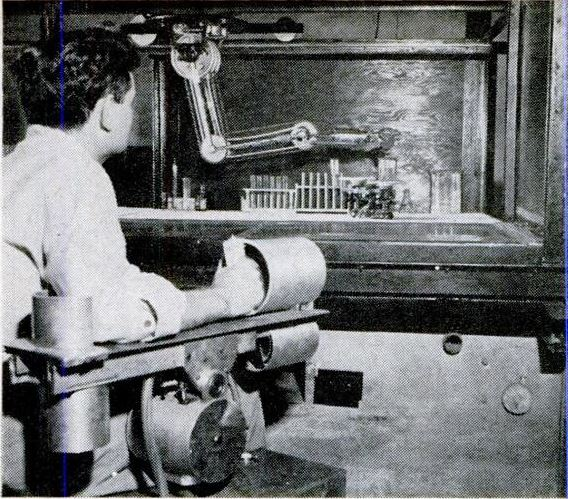
\includegraphics[width=6cm]{arm.jpg}
  \caption{Teleoperator mit radioaktivem Material, 1951}
  \label{fig:arm1}
\end{figure}

Die mechanischen Arme wurde noch in den 1950ern durch Schrittmotoren ersetzt und so ,,elektrifiziert''.
\end{frame}

\begin{frame}
\frametitle{Autonome mobile Roboter}
\begin{itemize}
\item  Unterwasserroboter (Wissenschaft, Bergung, \href{https://youtu.be/dF1Yb3Fa5sE?t=257}{Daten/Proben sammeln}) 
\item  \href{https://www.youtube.com/watch?v=5qqsMjy8Rx0}{Planetenrover}
\item  \href{https://www.youtube.com/watch?v=mhQixNlLF_k}{Arbeit in verseuchter Umgebung (Fukushima)}
\item  Bergung von Verletzten
\item  \href{https://www.youtube.com/watch?v=ujzjZuhE92g}{Pizza-Lieferservice} 
\item \textbf{Im Pizza-Roboter-Video war von Sensoren die Rede, welche kennst Du?}
\end{itemize}
\end{frame}

\begin{frame}
\frametitle{Vierbeinig läuft gut!}
\begin{figure}
  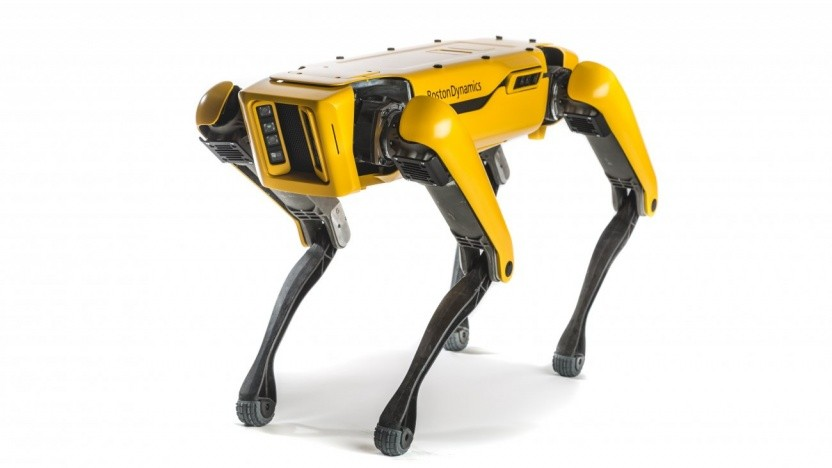
\includegraphics[width=\linewidth]{spot.png}
  \caption{Spot von Boston Dynamics}
  \label{fig:spot1}
\end{figure}

Ihr wollt \href{https://www.youtube.com/watch?v=OnWolLQSZic&feature=youtu.be}{Spot in Aktion} sehen? 
\end{frame}

% \begin{frame}
% \frametitle{Sensoren bei autonomen Robotern}
% \begin{itemize}
% \item   Entfernungssensor
% \item  Farbsensor
% \item   Schwarz-Weiss-Sensor $\Rightarrow$ Line-Follower
% \item   Magnetometer
% \item  interne Sensoren (Drehwinkel der Räder oder Poti eines Servos)
% \item Temperatur
% \item Gassensoren
% \item Radar, LIDAR, Kameras
% \end{itemize}
% \end{frame}

\begin{frame}
\frametitle{Wichtig: Wünsche an diese GTA und was bringt Ihr schon mit?}
\begin{itemize}
\item Wer baut gerne LEGO Technic?
\item Hat schon jemand Erfahrung mit Mindstorms oder anderen LEGO-Robotern?
\item  Was möchtet Ihr lernen?
\item  Was möchtet Ihr bauen?
\item   Was könnt Ihr schon?
\end{itemize}
\end{frame}


\end{document}
